\chapter{The Privacy Problem}
\label{ch:privacy-problem}

\begin{quote}
\textit{``Privacy is not about hiding wrongdoing. It's about protecting the ability to change and grow, to have different identities in different contexts, and to be free from the perfect memory of machines.''}
\end{quote}

\section*{Learning Objectives}
By the end of this chapter, you will:
\begin{itemize}
\item Understand what adversaries can observe in information systems
\item Recognize the three levels of privacy: data, access, and pattern
\item Learn why traditional approaches fail to provide practical privacy
\item Understand information-theoretic measures of privacy leakage
\item See how approximation can enable perfect observational privacy
\end{itemize}

\section{What Privacy Means in Computing}

Privacy in computing isn't about encryption alone—encrypted data that reveals access patterns still leaks information. Consider three levels of privacy:

\begin{enumerate}
\item \textbf{Level 1 - Data Privacy}: The content itself is protected
\item \textbf{Level 2 - Access Privacy}: Which data you access is hidden  
\item \textbf{Level 3 - Pattern Privacy}: Statistical patterns in access are obscured
\end{enumerate}

Most systems stop at Level 1. We're targeting Level 3.

\subsection{The Observation Problem}

Every interaction with a system creates observations:

\begin{lstlisting}[language=Python, caption={What servers observe even with encryption}]
class ServerObservations:
    def log_query(self, query_hash, timestamp):
        """Log every query - even hashed queries reveal patterns"""
        self.query_log.append({
            'hash': query_hash,
            'time': timestamp,
            'source_ip': get_client_ip(),
            'size': len(query_hash),
            'session_id': get_session()
        })
    
    def analyze_patterns(self):
        """Extract information from patterns"""
        # Frequency analysis
        freq = Counter(q['hash'] for q in self.query_log)
        
        # Temporal patterns  
        time_patterns = self.extract_time_patterns()
        
        # Correlation analysis
        correlations = self.find_query_pairs()
        
        # Session analysis
        user_sessions = self.group_by_session()
        
        return self.infer_user_interests(
            freq, time_patterns, correlations, user_sessions
        )
\end{lstlisting}

Even hashed queries leak information through:
\begin{itemize}
\item \textbf{Frequency}: Popular terms queried more often
\item \textbf{Timing}: Queries cluster around events
\item \textbf{Correlation}: Terms often searched together
\item \textbf{Volume}: Query rate reveals activity level
\item \textbf{Sessions}: Query sequences reveal investigation paths
\end{itemize}

\section{Case Study: The Research Scenario}

Let's make this concrete with a running scenario that illustrates the privacy challenges.

\begin{example}[Medical Research Database]
A medical researcher is investigating potential links between certain genetic markers and rare diseases. They need to search a genomic database for:
\begin{itemize}
\item Specific gene sequences
\item Patient cohorts with certain conditions
\item Statistical correlations
\item Treatment outcomes
\end{itemize}

Using a traditional search system, even with encryption:
\begin{lstlisting}[language=Python]
# Researcher's searches over one week
searches = [
    "BRCA1_mutation",        # Monday morning
    "breast_cancer_cohort",  # Monday afternoon
    "BRCA1_mutation",        # Tuesday (checking again)
    "ovarian_cancer_risk",   # Wednesday
    "BRCA1 AND ovarian",     # Thursday (correlation!)
    "prophylactic_surgery",  # Friday (treatment research)
]

# What adversary learns (even with hashing)
h1 = hash("BRCA1_mutation")     # Appears twice (high interest)
h2 = hash("breast_cancer_cohort") # Cancer research
h3 = hash("ovarian_cancer_risk")  # Multiple cancer types
# Correlation: h1 and h3 searched together (found connection!)
# Timeline: Moving from genes to treatment (hypothesis formed)
\end{lstlisting}

The server learns:
\begin{enumerate}
\item Researcher is investigating genetic cancer markers
\item Focus on BRCA1 gene (repeated searches)
\item Exploring multiple cancer types
\item Found correlation worth pursuing
\item Considering preventive treatments
\end{enumerate}

This could reveal:
\begin{itemize}
\item Competitive research directions
\item Potential patent applications
\item Personal health concerns
\item Institutional research priorities
\end{itemize}
\end{example}

\section{Traditional Approaches and Their Failures}

\subsection{Approach 1: Trusted Third Party}

\textbf{Idea}: Route queries through a trusted proxy that hides the source.

\textbf{Problems}:
\begin{itemize}
\item Single point of failure (technical and trust)
\item Proxy sees everything (insider threat)
\item Can be compromised or legally compelled
\item Doesn't hide patterns from database
\item Not scalable for global systems
\end{itemize}

\subsection{Approach 2: Homomorphic Encryption}

\textbf{Idea}: Compute on encrypted data without decrypting.

\begin{lstlisting}[language=Python, caption={Conceptual homomorphic search}]
# Conceptual homomorphic search
encrypted_query = homomorphic_encrypt("BRCA1")
encrypted_db = [homomorphic_encrypt(record) for record in database]
encrypted_results = search_on_encrypted(encrypted_query, encrypted_db)
results = homomorphic_decrypt(encrypted_results)
\end{lstlisting}

\textbf{Problems}:
\begin{itemize}
\item Computationally expensive (1000-1,000,000x slower)
\item Limited to specific operations
\item Still reveals access patterns
\item Ciphertext expansion (10-1000x larger)
\item Not practical for real-time systems
\end{itemize}

\subsection{Approach 3: Private Information Retrieval (PIR)}

\textbf{Idea}: Retrieve items without revealing which item.

\textbf{Two variants}:
\begin{enumerate}
\item \textbf{Information-theoretic PIR}: Perfect privacy but requires downloading entire database
\item \textbf{Computational PIR}: Smaller communication but relies on cryptographic assumptions
\end{enumerate}

\textbf{Problems}:
\begin{itemize}
\item Information-theoretic: Bandwidth = database size (impractical)
\item Computational: Still slow (100-10,000x overhead)
\item Doesn't handle complex queries well
\item No support for updates
\item Assumes non-colluding servers (multi-server PIR)
\end{itemize}

\subsection{Approach 4: Differential Privacy}

\textbf{Idea}: Add calibrated noise to hide individual contributions.

\textbf{Problems}:
\begin{itemize}
\item Designed for aggregate statistics, not point queries
\item Privacy budget depletes with queries
\item Noise accumulates, degrading utility
\item Doesn't hide query patterns
\item Complex parameter tuning
\end{itemize}

\section{The Fundamental Tradeoffs}

Every privacy system faces three competing demands:

\begin{center}
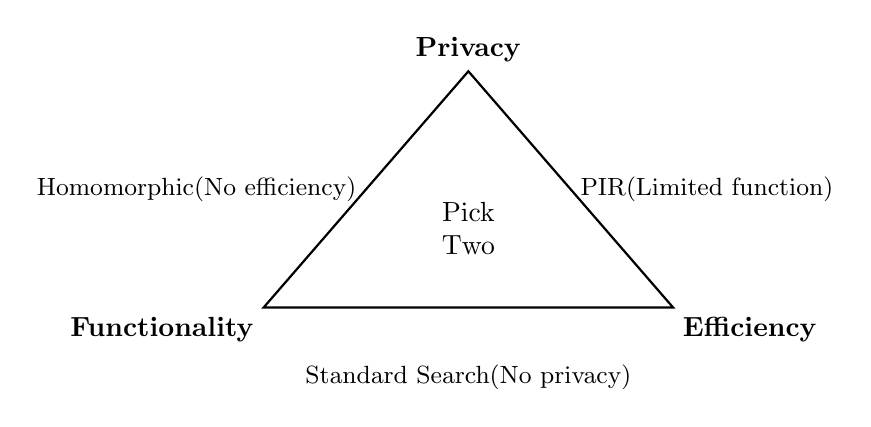
\begin{tikzpicture}[scale=2]
    % Triangle
    \coordinate (P) at (0,1.5);
    \coordinate (F) at (-1.3,0);
    \coordinate (E) at (1.3,0);
    
    % Draw triangle
    \draw[thick] (P) -- (F) -- (E) -- cycle;
    
    % Labels
    \node[above] at (P) {\textbf{Privacy}};
    \node[below left] at (F) {\textbf{Functionality}};
    \node[below right] at (E) {\textbf{Efficiency}};
    
    % Annotations
    \node[align=center] at (0,0.5) {Pick\\Two};
    
    % Examples on edges
    \node[left, font=\small] at (-0.65,0.75) {Homomorphic\\(No efficiency)};
    \node[right, font=\small] at (0.65,0.75) {PIR\\(Limited function)};
    \node[below, font=\small] at (0,-0.3) {Standard Search\\(No privacy)};
\end{tikzpicture}
\end{center}

Traditional approaches sacrifice one vertex:
\begin{itemize}
\item \textbf{Privacy + Functionality} → Terrible efficiency (homomorphic)
\item \textbf{Privacy + Efficiency} → Limited functionality (PIR)  
\item \textbf{Functionality + Efficiency} → No privacy (standard)
\end{itemize}

\section{Information Leakage: A Formal View}

Let's formalize privacy using information theory.

\subsection{Entropy and Information}

\begin{definition}[Entropy]
The entropy of a random variable $X$ with probability distribution $p(x)$ is:
$$H(X) = -\sum_{x} p(x) \log_2 p(x)$$
This measures the uncertainty (in bits) about $X$.
\end{definition}

\begin{definition}[Conditional Entropy]
The conditional entropy of $X$ given $Y$ is:
$$H(X|Y) = -\sum_{x,y} p(x,y) \log_2 p(x|y)$$
This measures remaining uncertainty about $X$ after observing $Y$.
\end{definition}

\begin{definition}[Mutual Information]
The mutual information between query $Q$ and observations $O$ is:
$$I(Q; O) = H(Q) - H(Q|O) = H(O) - H(O|Q)$$
This measures how much information $O$ reveals about $Q$.
\end{definition}

Perfect privacy requires $I(Q; O) = 0$, meaning observations tell us nothing about queries.

\subsection{Sources of Leakage}

\begin{theorem}[Frequency Leakage]
Given query frequency $p(q)$ and observation probability $p(o|q)$, Bayes' theorem gives:
$$P(q | o) = \frac{P(o|q) \cdot P(q)}{\sum_{q'} P(o|q') \cdot P(q')}$$
More frequent queries are more likely given an observation.
\end{theorem}

\begin{theorem}[Correlation Leakage]
If queries $q_1, q_2$ frequently co-occur:
$$P(q_1, q_2 | o_1, o_2 \text{ together}) > P(q_1) \cdot P(q_2)$$
violating independence and revealing relationships.
\end{theorem}

\begin{theorem}[Temporal Leakage]
Time-dependent query distributions:
$$P(q | t) \neq P(q)$$
reveal context through timing patterns.
\end{theorem}

\subsection{The Distinguishability Problem}

An adversary succeeds if they can distinguish between hypotheses:

\begin{definition}[Privacy Game]
\begin{enumerate}
\item Adversary chooses two query sequences $Q_0, Q_1$
\item System randomly picks $b \in \{0,1\}$ and executes $Q_b$
\item Adversary observes $O$ and outputs guess $b'$
\item Adversary wins if $b' = b$
\end{enumerate}
Privacy fails if $\Pr[\text{win}] > \frac{1}{2} + \text{non-negligible}$.
\end{definition}

\section{Requirements for True Privacy}

Based on these failures, a truly private system must:

\begin{enumerate}
\item \textbf{Hide Access Patterns}: Which items are accessed must be obscured
\item \textbf{Provide Uniform Representations}: All queries should look identical
\item \textbf{Break Correlations}: Related queries shouldn't appear related
\item \textbf{Obscure Frequencies}: Common and rare queries indistinguishable
\item \textbf{Maintain Efficiency}: Still practical for real use
\item \textbf{Support Full Functionality}: Complex queries, updates, etc.
\end{enumerate}

This seems impossible! How can queries look identical yet return different results?

\section{The Bernoulli Insight}

Here's the key realization: \textit{approximate representations can provide exact privacy}.

Instead of making queries indistinguishable while preserving exact functionality (impossible), we:
\begin{enumerate}
\item Accept approximate results (Bloom filter style)
\item Make the approximations truly uniform
\item Hide all patterns in the noise
\end{enumerate}

\begin{proposition}[The Privacy-Approximation Exchange]
A system can achieve perfect observational privacy if:
\begin{enumerate}
\item All queries map to uniform random representations
\item Results are approximate with bounded error $\varepsilon$
\item Errors are independent of query content
\item The representation space is large enough ($|R| \gg |Q|$)
\end{enumerate}
\end{proposition}

This leads to our framework:

\begin{center}
\begin{tikzpicture}[scale=0.9]
    % Input
    \node[draw, rectangle] (input) at (0,0) {Query $q$};
    
    % Encoding
    \node[draw, rectangle, fill=blue!20] (encode) at (2.5,0) {Bernoulli\\Encode};
    \draw[->] (input) -- (encode);
    
    % Oblivious representation
    \node[draw, rectangle, fill=red!20] (oblivious) at (5,0) {Uniform\\$\tilde{q}$};
    \draw[->] (encode) -- (oblivious);
    
    % Server processing
    \node[draw, rectangle] (server) at (7.5,0) {Server};
    \draw[->] (oblivious) -- (server);
    
    % Results
    \node[draw, rectangle, fill=red!20] (results) at (7.5,-2) {Noisy\\$\tilde{r}$};
    \draw[->] (server) -- (results);
    
    % Decoding
    \node[draw, rectangle, fill=blue!20] (decode) at (5,-2) {Decode};
    \draw[->] (results) -- (decode);
    
    % Output
    \node[draw, rectangle] (output) at (2.5,-2) {Result\\$r \pm \varepsilon$};
    \draw[->] (decode) -- (output);
    
    % Adversary
    \node[draw, ellipse, fill=gray!30] (adversary) at (6.5,1.5) {Adversary};
    \draw[dashed, ->] (oblivious) -- (adversary);
    \draw[dashed, ->] (server) -- (adversary);
    \node[right] at (7.5,1.5) {\small Sees uniform noise!};
\end{tikzpicture}
\end{center}

\section{Legal and Ethical Considerations}

\subsection{Regulatory Landscape}

Modern privacy regulations impose strict requirements:

\begin{itemize}
\item \textbf{GDPR (EU)}: Data minimization, purpose limitation, privacy by design
\item \textbf{CCPA (California)}: Right to know, delete, opt-out
\item \textbf{HIPAA (Healthcare)}: Minimum necessary standard
\item \textbf{Sector-specific}: Financial (PCI-DSS), Education (FERPA)
\end{itemize}

Our approach helps compliance by ensuring queries reveal nothing.

\subsection{Ethical Dimensions}

Privacy-preserving systems raise ethical questions:
\begin{itemize}
\item \textbf{Dual use}: Same techniques could hide malicious activity
\item \textbf{Accountability}: How to audit while preserving privacy?
\item \textbf{Transparency}: Users should understand privacy guarantees
\item \textbf{Equity}: Privacy tools shouldn't only benefit the privileged
\end{itemize}

\section{Exercises}

\begin{enumerate}
\item \textbf{Leakage Analysis}: Given a log of 1000 hashed queries where hash $h_1$ appears 300 times and $h_2$ appears 3 times, what can you infer about the underlying query distribution?

\item \textbf{Correlation Detection}: If $P(h_1) = 0.1$, $P(h_2) = 0.05$, but $P(h_1, h_2 \text{ within 1 minute}) = 0.04$, calculate the correlation coefficient. What might this suggest?

\item \textbf{Privacy Metrics}: Calculate the mutual information $I(Q; O)$ for a system where each query $q_i$ has frequency $p_i$ and is correctly observed with probability $0.9$.

\item \textbf{Tradeoff Exploration}: Design a system for private web search. Which vertex of the privacy-functionality-efficiency triangle would you sacrifice and why?

\item \textbf{Attack Simulation}: Write code to distinguish between random queries and queries following a theme using only frequency analysis. Test on real query logs.
\end{enumerate}

\section{Chapter Summary}

Privacy in computing isn't just about hiding data—it's about hiding access patterns, correlations, and frequencies. Traditional approaches fail because they try to preserve exact functionality while achieving privacy, hitting fundamental impossibility results.

Our key insight: approximate data structures that introduce controlled errors can achieve perfect observational privacy. By making all queries look like uniform random noise, we hide not just what you're searching for, but that you're searching at all.

The price? Small, bounded errors in results. The reward? Practical privacy that works at scale.

Next, we'll build this vision into reality, creating your first oblivious system that provides true privacy through the power of probabilistic approximation.

\section{Further Reading}

\begin{itemize}
\item Goldreich, O. \& Ostrovsky, R. (1996). ``Software protection and simulation on oblivious RAMs''
\item Gentry, C. (2009). ``A fully homomorphic encryption scheme''
\item Islam, M. et al. (2012). ``Access pattern disclosure on searchable encryption''
\item Cash, D. et al. (2015). ``Leakage-abuse attacks against searchable encryption''
\item Grubbs, P. et al. (2018). ``Pump up the volume: Practical database reconstruction from volume leakage''
\end{itemize}